\documentclass[twocolumn,10pt]{article}

\usepackage[margin=1.8cm]{geometry}
\usepackage{amsmath, amssymb}
\usepackage{graphicx}
\usepackage{physics}
\usepackage{bm}
\usepackage{authblk}
\setlength{\columnsep}{0.6cm}

%\title{\textbf{Entanglement-Dynamic Topology Enables Programmable Quantum Resources}}
% ============================================================
% TITLE
% ============================================================

\title{
Programmable Quantum Resource Manifolds via Entanglement-Dynamic Topology
}

\author[1]{Hang Hu \thanks{Correspondence to: hang.hu@cnrc-nrc.gc.ca}}
\affil[1]{Digital Technologies, National Research Council of Canada, 222 College Street, Toronto, ON M5T 3J1, Canada}
\author[1]{Hsu Kiang Ooi}
\author[2]{Anguang Hu \thanks{Correspondence to: anguang.hu@forces.gc.ca}}
\affil[2]{Suffield Research Centre, Defence Research and Development Canada, PO Box 4000 Station Main, Medicine Hat, Alberta T1A 8K6, Canada}

\date{\today}

\begin{document}

\twocolumn[
\maketitle
\begin{center}
\small
Correspondence to: hang.hu@cnrc-nrc.gc.ca; anguang.hu@forces.gc.ca
\end{center}
\vspace{0.5em}
\begin{center}
\begin{minipage}{0.95\textwidth}
\small
\textbf{Abstract.}
Quantum technologies rely on entanglement, coherence, superposition, and interference as fundamental resources, yet conventional approaches seek to maximize these quantities globally, leading to exponential complexity associated with Hilbert-space scaling. Here we introduce Entanglement–Dynamic Topology (EDT) as a framework for programmable quantum resource engineering, in which quantum resources are organized into finite, geometry-aligned manifolds rather than distributed across the full Hilbert space. We show that EDT emerges from non-adiabatic coupling between electronic and lattice degrees of freedom, where second-order variations of electronic energies with respect to normal-mode coordinates generate curvature fields that act as sources of entanglement and organize interference through geometric and topological structure. This connects EDT directly to the microscopic physics of electron–phonon interactions, including the Bardeen–Pines formalism and the foundations of BCS theory. We demonstrate a data-driven identification of EDT in K$_3$C$_{60}$, where curvature-resolved band structure reveals a finite momentum interval in which paired branches admit a consistent local quadratic description. We further show that this regime emerges generically in a minimal dynamical model, where loop-induced operator spreading remains structured and compatible with persistent many-body correlations, and that it is robust under parameter variation, bounded circuit complexity, and approximate implementation. Finally, we establish an experimental realization in NV-center sensing, where optimal performance arises within a finite control regime balancing competing quantum resources. These results establish a new paradigm in which quantum advantage arises not from Hilbert-space scaling, but from the controlled organization of quantum resources into structured dynamical manifolds generated by microscopic interactions.
\end{minipage}
\end{center}
\vspace{1em}
]

% ============================================================
\section*{Introduction}


Quantum computation, sensing, and materials design fundamentally depend on the controlled use of quantum resources, including entanglement, coherence, superposition, and interference~\cite{NielsenChuang,Horodecki2009,Streltsov2017}. In most current approaches, these resources are treated as quantities to be maximized, leading naturally to strategies that explore increasingly large Hilbert spaces~\cite{Preskill2018,Arute2019}. While powerful in principle, this paradigm introduces severe scaling challenges and often obscures the physical structure underlying useful quantum dynamics~\cite{Eisert2010,Altman2015}.

An alternative perspective is that quantum advantage arises not from the size of Hilbert space, but from the organization of quantum resources within it~\cite{Amico2008,Swingle2018}. In this view, the central problem is not to generate maximal entanglement, but to engineer entanglement that is structured, localized, and aligned with the geometry of the task~\cite{Verstraete2008,Orus2014}. This shift reframes quantum control as a problem of resource organization rather than resource amplification. In this sense, useful quantum dynamics are not those that explore the largest possible state space, but those that remain confined to structured manifolds where entanglement, interference, and correlation are jointly optimized~\cite{KimHuse2013,Choi2016}.

Here we use Entanglement--Dynamic Topology (EDT) as an organizing framework for identifying finite, structured dynamical regimes in quantum materials and their circuit-level analogues. Building on recent studies of curvature-driven and topologically structured quantum dynamics~\cite{Hu2024_ACP,Hu2025_APQ,Hu2026_JPCM}, EDT is used here to connect measurable electronic-structure features, such as paired curvature and local quadratic stability, with controllable dynamical signatures relevant to quantum-resource design.

EDT describes a finite regime in which symmetry-induced structure, interaction-driven mixing, topological organization, and controllable dynamics overlap in a measurable way. In this view, structure captures the reduction of accessible state space by symmetry~\cite{Wigner1959,Georgi1999}, interaction, including non-adiabatic electron--phonon coupling, provides a mechanism for mixing states and redistributing correlations~\cite{Mead1979,Yarkony1996}. Topology organizes the response through robust features such as nodes, degeneracies, and winding-like configurations in parameter space~\cite{Berry1984,Xiao2010}. Dynamics makes this response observable and tunable through changes in band energies, electronic potentials, or circuit observables~\cite{Bukov2015,Eckardt2017}. Thus, in this work EDT is not introduced as a universal classification of quantum resources, but as an operational framework for locating finite regime where these four features are simultaneously visible.

Within this regime, quantum dynamics exhibit coherent, structured behavior, while outside it the dynamics become either weakly correlated or overdriven and incoherent~\cite{Larkin1969,Swingle2018}. 

To connect this framework to real physical systems, we apply this method to K$_3$C$_{60}$ as a representative molecular solid with strong electron--phonon coupling and correlated electronic behavior~\cite{Gunnarsson1997,Capone2009}. We analyze curvature-resolved band structure and show that EDT appears as a finite momentum interval in which paired curvature branches admit a consistent local quadratic description (Fig.~2). This provides an operational criterion for detecting EDT directly from microscopic electronic-structure observables. 

Figure~\ref{fig:materials_summary} summarizes the broader archived materials comparison that frames this diagnostic. It compares the extracted EDT-window widths and bootstrap confidence intervals for K$_3$C$_{60}$, Na, V, YBa$_2$Cu$_3$O$_7$, and LaH$_{10}$ using the same paired-curvature workflow. The detailed branch-resolved panels are kept in the SI, while the main-text summary makes clear that finite EDT windows are reproducible across materials but not universal in size.

This regime-based perspective provides a robust and experimentally meaningful foundation for quantum resource engineering, in contrast to approaches that rely on asymptotic scaling or finely tuned optimality.

We then show that this regime arises generically in a minimal dynamical model (Fig.~3), where loop-induced operator spreading remains structured and compatible with persistent many-body correlation, and that it remains robust under parameter variation, bounded circuit complexity, and approximate implementation (Fig.~4)~\cite{Lloyd1996,Childs2019}. 

More broadly, EDT enables a programmable resource paradigm in which target quantum resources are mapped onto finite manifolds and compiled into physical control primitives. This shifts the focus of quantum science from Hilbert-space scaling to resource structuring, with implications for quantum computing, sensing, and geometry-aligned algorithm design~\cite{Preskill2018,Verstraete2008}.



\section*{\raggedright Microscopic Origin of Entanglement-Dynamic Topology}

The origin of EDT begins with symmetry, which imposes a fundamental organization on quantum states. Symmetry decomposes Hilbert space into constrained manifolds, restricting dynamics to geometry-aligned subspaces~\cite{Wigner1959,Georgi1999}. This structural reduction concentrates quantum resources into physically meaningful sectors, replacing uniform Hilbert-space exploration with a structured resource landscape. In this sense, symmetry defines the geometric scaffold on which quantum dynamics unfold.

Interactions provide the mechanism for generating and redistributing quantum resources within this scaffold. In particular, non-adiabatic coupling (NACT), such as electron--phonon interaction, induces mixing between electronic states through nuclear motion~\cite{Mead1979,Yarkony1996}. Near degeneracies and band crossings, this mixing becomes enhanced, giving rise to strong second-order modulation of band energies. These effects are captured by the curvature
\begin{equation}
\kappa_{n\alpha} = \frac{\partial^2 E_n}{\partial Q_\alpha^2},
\end{equation}
which quantifies the response of electronic structure to lattice motion and serves as a microscopic source of entanglement. Unlike adiabatic descriptions, which treat electronic states as isolated, these non-adiabatic processes dynamically generate correlated quantum states that extend across the structured manifold~\cite{BornOppenheimer1927}. This curvature-based and topological organization of quantum dynamics has been previously identified in compressed metallic systems and quantum bonding regimes~\cite{Hu2024_ACP,Hu2025_APQ,Hu2026_JPCM}.

The combination of symmetry and interaction gives rise to a topological organization of quantum resources. The NACT fields
\begin{equation}
A^{(\alpha)}_{mn} = \langle m | \partial_{Q_\alpha} | n \rangle
\end{equation}
define a Berry-like connection in parameter space, whose associated curvature encodes the geometric structure of the coupled electronic manifold~\cite{Berry1984,Xiao2010}. Near degeneracies, this structure manifests as nodes, poles, and vortex-like features that act as organizing centers for quantum dynamics, stabilizing interference and defining pathways along which quantum resources are concentrated and transported.

Crucially, these structures are dynamical. Time-dependent modulation of band energies and electronic potentials renders the resource manifold controllable. External drives, lattice distortions, and environmental interactions reshape the curvature landscape, enabling preparation, steering, and stabilization of quantum resources~\cite{Bukov2015,Eckardt2017}. This dynamical aspect transforms the structured manifold into a programmable object.

These ingredients admit an effective description in terms of curvature-mediated interactions. 

Starting from the electron--phonon Hamiltonian
\begin{equation}
H = H_e(\mathbf{r};\{Q_\alpha\}) + \sum_\alpha \left(\frac{P_\alpha^2}{2M_\alpha} + \frac{1}{2} M_\alpha \omega_\alpha^2 Q_\alpha^2\right),
\end{equation}
non-adiabatic effects arise from the dependence of the electronic Hamiltonian on normal-mode coordinates $Q_\alpha$~\cite{BornOppenheimer1927,Mead1979,Yarkony1996}. Expanding $H_e$ to second order,
\begin{equation}
H_e(\{Q_\alpha\}) \approx H_e^{(0)} + \sum_\alpha Q_\alpha \,\partial_\alpha H_e
+ \frac{1}{2}\sum_{\alpha\beta} Q_\alpha Q_\beta \,\partial_\alpha \partial_\beta H_e,
\end{equation}
and projecting onto an adiabatic electronic basis $\{|n\rangle\}$ yields NACT matrix elements
\begin{equation}
A^{(\alpha)}_{mn} = \langle m | \partial_{Q_\alpha} | n \rangle,
\end{equation}
which generate off-diagonal mixing and geometric phases~\cite{Mead1979,Berry1984}. Eliminating fast phonon coordinates (e.g., via a Born--Oppenheimer breakdown or polaron/Schrieffer--Wolff treatment) produces an effective electronic Hamiltonian with curvature-mediated interactions~\cite{SchriefferWolff1966,LangFirsov1962},
\begin{equation}
H_{\mathrm{eff}} \simeq H_0 + \sum_{\langle i,j\rangle} J_{ij}\, Z_i Z_j
+ \sum_p \lambda_p\, W_p,
\end{equation}
where $J_{ij}$ arises from second-order (curvature) processes and $W_p$ denotes loop (plaquette) operators generated by multi-mode interference of NACT fields.

In momentum space, the same physics appears as curvature of band energies with respect to normal-mode coordinates in Eq. (1), which acts as a source of entanglement and defines the structured manifold on which dynamics are confined~\cite{BardeenPines1955,BCS1957}. The loop terms $W_p$ encode the holonomy of the NACT connection, linking curvature to interference-stabilized dynamics that define the EDT regime~\cite{Berry1984,Xiao2010}.

At the operational level, when curvature is smoothly varying and geometrically coherent, paired structures admit a stable quadratic description, yielding a finite EDT window in which quantum resources are localized and robust. Outside this regime, either curvature is too weak to generate correlations or too sharply varying to support a stable manifold, leading to weakly correlated or overdriven dynamics~\cite{Larkin1969,Swingle2018}.


Importantly, this structure is not limited to materials systems. The same Hamiltonian structure can be implemented in quantum circuits through Trotterized evolution of local interactions and plaquette terms, providing a direct realization of EDT dynamics in gate-based architectures (see Supplementary Information (SI), Sec.~S7)~\cite{Lloyd1996,Childs2019}. This establishes EDT as a general framework spanning from electronic structure, to quantum information processing.
 

\section*{\raggedright Applications: Computation, Measurement, and Sensing}

A key feature of EDT is that quantum resources are not static quantities, but dynamically structured and controllable through the underlying physical degrees of freedom~\cite{Amico2008,Eisert2010}. In contrast to conventional approaches that treat entanglement and coherence as globally distributed, EDT identifies regimes in which these resources are localized within finite, geometry-aligned manifolds that evolve under controlled modulation~\cite{Verstraete2008,Orus2014}.

Figure~\ref{fig:k3c60_edt} provides a direct, data-driven realization of this principle in K$_3$C$_{60}$~\cite{Gunnarsson1997,Capone2009}. The electronic band structure near the Fermi level [Fig.~\ref{fig:k3c60_edt}(a)] exhibits paired branches reflecting the combined effects of symmetry and interaction-induced correlations. While band crossings indicate the presence of coupling, the defining signature of EDT emerges at the level of curvature.

The curvature of the band energies with respect to the control coordinate [Fig.~\ref{fig:k3c60_edt}(b)] reveals localized regions of enhanced second-order response, corresponding to strong non-adiabatic coupling~\cite{Mead1979,Yarkony1996}. These curvature features are not uniformly distributed across momentum space, but instead form spatially localized structures. This localization provides direct evidence that quantum resources are concentrated within finite regions rather than distributed across the full Brillouin zone (see SI, Sec.~S4).

A more precise characterization is obtained by examining paired curvature branches near the crossing region. As shown in Fig.~\ref{fig:k3c60_edt}(c), these branches admit a consistent local quadratic description within a finite momentum interval. This defines an intrinsic curvature scale $k_0$ and a corresponding core region $\Delta k_{\mathrm{core}}$, within which the two branches remain mutually compatible. The existence of this quadratic structure reflects an underlying geometric constraint imposed by non-adiabatic coupling and band topology~\cite{Berry1984,Xiao2010}.

This observation leads to an operational definition of the EDT regime. As shown in Fig.~\ref{fig:k3c60_edt}(d), the EDT window $\Delta k_{\mathrm{EDT}}$ is defined as the maximal momentum interval over which the paired curvature branches admit a stable quadratic description and remain within a prescribed residual threshold (see SI, Sec.~S2). Within this window, curvature, coupling, and topology combine to produce a structured dynamical regime in which quantum resources are both generated and stabilized. Outside this region, the quadratic description breaks down, signaling a transition to either weakly correlated or overdriven dynamics~\cite{Larkin1969,Swingle2018}.

The finite extent of $\Delta k_{\mathrm{EDT}}$ is a central feature of the EDT framework. Unlike critical-point descriptions, which rely on singular behavior, the EDT regime occupies a finite interval in parameter space, providing intrinsic robustness to perturbations~\cite{Altman2015}. This implies that quantum resources can be accessed and manipulated without fine tuning, and that the structured manifold defines a stable operating window for quantum dynamics.

From the perspective of quantum resource engineering, the relevant degrees of freedom are those associated with the structured manifold defined by $\Delta k_{\mathrm{EDT}}$, rather than the full Hilbert space. This enables a shift from global resource maximization to local resource concentration, in which entanglement, coherence, superposition, and interference are confined to physically meaningful regions aligned with the underlying geometry.

More broadly, Fig.~\ref{fig:k3c60_edt} establishes a direct connection between microscopic electronic structure and programmable quantum resources. The identification of curvature pairing, a local quadratic structure, and a finite EDT window provides a concrete, data-driven criterion for detecting EDT in real materials. This bridges the gap between physical observables and functional quantum capability, and demonstrates how structured dynamics can be harnessed for quantum computation, measurement, and sensing. A corresponding quantum circuit realization of these dynamics, based on a minimal plaquette model, is provided in SI, Sec.~S7~\cite{Lloyd1996,Childs2019}. Additional archived material examples are collected in SI, Sec.~S4.


Having identified EDT as a finite structured window in the material response, we next ask whether the same type of dynamics can be realized in a programmable model. We consider a four-qubit plaquette system, which can be interpreted as a quantum gyroscopic model. Local interactions and plaquette terms generate loop-organized evolution in Hilbert space, while the plaquette operator acts as a non-local diagnostic of collective dynamics. This construction provides a compact setting for testing controlled operator spreading, persistent many-body correlation, and approximate circuit implementation within the EDT regime. Details of the Trotterized circuit realization are provided in SI, Sec.~S7.


Figures~3 and 4 show that useful quantum dynamics arise not from maximal operator spreading, but from a finite regime in which spreading remains structured and compatible with persistent many-body correlations~\cite{Swingle2018,Choi2016}. Increasing interaction strength or circuit depth beyond this regime drives the system into an overdriven phase in which coherence and correlation degrade~\cite{Altman2015}.

The Trotterized circuit realization explicitly implements the interplay between local interactions and loop-induced terms that define the EDT regime. In particular, the plaquette operator $Z_0 Z_1 Z_2 Z_3$ generates non-local correlations that cannot be reduced to pairwise interactions, producing structured entanglement aligned with the underlying geometry. This demonstrates that EDT is not only a property of electronic structure, but also a programmable feature of quantum circuits (see SI, Sec.~S7)~\cite{Lloyd1996,Childs2019,Trotter1959,Suzuki1990}.

Furthermore, the resulting circuits enable direct measurement of dynamical diagnostics such as out-of-time-order correlators (OTOCs), which probe operator spreading~\cite{Larkin1969,Swingle2018}. In the EDT regime, OTOCs exhibit structured growth and saturation consistent with a finite, geometry-aligned entanglement manifold.

From this perspective, quantum computation can be understood as controlled evolution within a structured dynamical manifold. The optimal operating point is not one of maximal entanglement, but one in which operator growth, correlation retention, and temporal organization are jointly optimized. The robustness of this regime under parameter variation and approximate implementation (Fig.~4) indicates that it can be targeted in realistic quantum architectures~\cite{Preskill2018,Arute2019}.

The same regime structure governs quantum measurement. In many-body systems, measurement sensitivity depends on accessing non-local operators while preserving coherence. The EDT regime identified in Fig.~3 provides precisely this balance: operator spreading is sufficiently strong to probe extended correlations, yet sufficiently structured to preserve measurable signals at late times~\cite{KimHuse2013,Choi2016}.

This establishes a general principle for quantum measurement: optimal sensitivity is achieved within a finite regime where operator growth and correlation persistence coexist, rather than at maximal scrambling~\cite{Swingle2018}.

The NV-center platform provides a concrete experimental realization of EDT as a quantum resource engineering problem~\cite{Degen2017,Barry2020}. In NV--XY8 sensing protocols, performance is governed by a structured combination of resource factors, including filter gain $G(f)$, coherence time, pulse fidelity, and readout contrast. As shown in Fig.~\ref{fig:fig5_nvdemo}, these quantities do not improve monotonically with control parameters such as pulse number $N$ or spacing $\tau$. Instead, an optimal operating point emerges as a finite regime in which signal amplification, coherence preservation, and control accuracy are balanced~\cite{Casola2018}.

This behavior is directly analogous to the EDT regime identified in Figs.~3 and 4. Increasing control strength enhances sensitivity through improved filter response, but also accelerates decoherence and accumulates control errors. As a result, sensing performance exhibits a maximum within a finite window rather than at extreme parameter values. Within this regime, the sensor dynamics remain aligned with a structured manifold in control space, enabling both selective response and coherence localization~\cite{Degen2017,Barry2020}.

\section*{Discussion}

The present framework builds on several strands of research showing that useful quantum behavior is often organized by structure rather than by unrestricted access to the full Hilbert space. In condensed-matter physics, non-adiabatic coupling, curvature, electron--phonon interactions, and geometric phase effects have long been used to describe how lattice motion reshapes electronic structure~\cite{Mead1979,Yarkony1996,Giustino2017}. In quantum information, tensor-network methods and symmetry-resolved constructions, including Schur transforms and Clebsch--Gordan decompositions, similarly exploit the fact that many-body states often occupy structured subspaces~\cite{Schollwock2011,Bacon2006}. Recent quantum algorithms, including variational quantum eigensolvers and quantum approximate optimization algorithms, further emphasize the value of tailoring quantum dynamics to the structure of the target problem~\cite{Peruzzo2014,Farhi2014}. The systems studied here connect these ideas in a common setting: microscopic curvature and interaction define finite organized regimes, while dynamical models and circuit implementations test whether those regimes can support controllable quantum behavior.

Across our materials analysis (Fig.~2), minimal dynamical models (Fig.~3), and implementation-level considerations (Fig.~4), we show that useful quantum dynamics can be identified and extracted from such finite organized regimes. In these regimes, structure, interaction, topology, and dynamics act together to produce controllable behavior, without requiring maximal entanglement or unrestricted exploration of Hilbert space~\cite{Amico2008,Eisert2010}. In many quantum-engineering settings, increasing interaction strength, circuit depth, or entanglement can improve performance only up to a point~\cite{Preskill2018}. The results here support this finite-window perspective: beyond the structured regime, dynamics can become overdriven, leading to degradation of coherence, correlation stability, or implementation accuracy. This reveals a practical trade-off: the same interactions that generate useful quantum resources can also destabilize them when pushed beyond the organized regime~\cite{Altman2015,Swingle2018}.

The data-driven identification of EDT in K$_3$C$_{60}$ (Fig.~2) demonstrates that this regime arises directly from microscopic electronic structure~\cite{Gunnarsson1997,Capone2009}. The existence of a finite curvature-defined window $\Delta k_{\mathrm{EDT}}$ shows that non-adiabatic coupling naturally organizes quantum resources into localized regions of momentum space~\cite{Mead1979,Yarkony1996}. This provides a physical origin for structured quantum dynamics and suggests that similar regimes may be present across a wide range of correlated materials.

The broader comparison in Fig.~\ref{fig:materials_summary} sharpens that point. The fulleride reference is not simply reproduced with the same scale in every material: the selected Na and V metallic pairs support broader extracted windows, whereas the selected YBa$_2$Cu$_3$O$_7$ and LaH$_{10}$ subsets remain more localized. The comparison of widths and bootstrap intervals makes the central point explicit: the diagnostic is portable across materials, but the finite window itself is material dependent.

The curvature-based origin of EDT also connects directly to the microscopic theory of superconductivity. In the Bardeen--Pines formulation, electron--phonon interactions renormalize the electronic potential through dynamical screening, producing an effective attractive interaction that underlies BCS pairing~\cite{BardeenPines1955,BCS1957}. These interactions arise from the same dependence of electronic energies on lattice coordinates that generates the non-adiabatic coupling fields considered here.

From the EDT perspective, the key quantity is the second-order response of electronic energies to normal-mode coordinates in Eq. (1), which captures curvature induced by lattice dynamics. While in conventional superconductivity this curvature contributes to pairing amplitudes, EDT interprets it more broadly as a generator of structured quantum resource manifolds. In particular, regions of enhanced curvature define finite domains in parameter space where electronic states are strongly coupled, interference is stabilized, and correlated dynamics are supported~\cite{Giustino2017}.

These results motivate a broader comparative analysis in which superconducting systems are assessed not only through the magnitude of their electron--phonon coupling, but also through the geometry and stability of their curvature response. In this view, systems with smooth, extended curvature structures may be more likely to support finite EDT-like windows, whereas systems with sharply varying or fragmented curvature may fail to form stable local manifolds even when coupling is strong. Establishing this connection quantitatively will require broader cross-material studies and direct comparison with conventional superconducting descriptors such as electron--phonon coupling constants, phonon linewidths, and superconducting transition temperatures.

From a dynamical perspective, the minimal plaquette model (Fig.~3) shows that the EDT regime is characterized by the coexistence of operator spreading and persistent many-body correlations~\cite{Choi2016,KimHuse2013}. This distinguishes EDT from both weakly interacting systems, where dynamics remain local, and strongly driven systems, where coherence is rapidly lost. Instead, EDT occupies an intermediate regime in which interference is stabilized by topology and constrained by symmetry, leading to dynamically organized entanglement~\cite{Swingle2018}.

The scaling and implementation results (Fig.~4) further demonstrate that this regime is operationally robust. The persistence of the optimal loop strength $\lambda^\star$ and the EDT score under parameter variation and approximate Trotterization indicates that the regime is not fine-tuned~\cite{Lloyd1996,Childs2019}. This establishes EDT as a practical design principle for quantum technologies, guiding the selection of operating conditions in both digital and analog platforms.

This connection is natural from the perspective of quantum algorithms. Variational quantum eigensolvers and quantum approximate optimization algorithms already restrict the accessible dynamics to parametrized, problem-adapted circuit families~\cite{Peruzzo2014,Farhi2014}. Tensor-network methods similarly exploit the fact that many relevant many-body states occupy structured regions of Hilbert space rather than arbitrary states~\cite{Schollwock2011}. EDT provides a complementary physical route to this idea: instead of imposing structure only through an ansatz or representation, it identifies structured manifolds from microscopic ingredients such as curvature, non-adiabatic coupling, symmetry, and local dynamical stability. This suggests a route toward physically informed quantum algorithms in which circuit structure, variational ansatz design, or Hamiltonian simulation choices are guided by the geometry of the underlying resource window.

The NV-center sensing results (Fig.~5) extend the EDT perspective from identifying structured dynamical windows to engineering them in an experimental quantum platform~\cite{Degen2017,Barry2020}. In NV--XY8 protocols, sensing performance is controlled by a balance among filter gain, coherence time, pulse fidelity, and readout contrast. As shown in Fig.~5, the best sensitivity occurs within a finite control regime where these factors are jointly optimized, rather than at the maximum value of any single resource. This provides an engineering interpretation of EDT: useful performance is obtained by tuning the system into a stable operational window where competing quantum resources remain simultaneously effective~\cite{Casola2018}.

The NV platform therefore provides a practical extension of the EDT picture: the finite-regime behavior identified in electronic structure and minimal models also appears in an experimentally accessible sensing protocol. This supports the use of EDT as a physically motivated organizing framework for analyzing quantum resources, rather than as a universal classification scheme. A corresponding quantum circuit realization of these dynamics, based on a minimal four-qubit plaquette model, provides a direct mapping between EDT Hamiltonian structure and gate-level operations (see SI, Sec.~S7)~\cite{Lloyd1996,Childs2019}.

Taken together, these results support a broader perspective on programmable quantum systems: the relevant task is often not to access the largest possible Hilbert space, but to identify and control finite regions in which quantum resources are structured, stable, and useful.

More generally, EDT provides a bridge between condensed-matter physics and quantum information~\cite{NielsenChuang,Amico2008}. The same curvature that governs pairing interactions also defines the structure of entanglement and interference in Hilbert space~\cite{Berry1984,Xiao2010}. In this sense, superconducting materials may be viewed as natural platforms in which structured quantum resource regimes emerge from microscopic interactions, offering new routes for both understanding and engineering quantum functionality~\cite{BCS1957,Giustino2017}. Additional examples across materials classes are provided in SI, Sec.~S4, with temperature-dependent effects discussed in Sec.~S5.

A central aspect of this framework is the role of degeneracy in shaping the response of electronic energies to lattice dynamics. While electron--phonon interactions have been extensively studied within the Bardeen--Pines formalism and BCS theory~\cite{BardeenPines1955,BCS1957}, these approaches do not explicitly formulate the second-order response of electronic energies within degenerate or near-degenerate manifolds as a structured geometric object. Here, we show that this curvature defines a finite, geometry-aligned manifold that organizes entanglement, interference, and dynamical response. The present results therefore provide a data-driven realization of this structure, supported by comprehensive calculations presented in the SI.



\section*{Conclusion and Outlook}

We have introduced EDT as a framework for identifying finite, geometry-aligned regimes in which quantum resources remain structured and controllable. By combining electronic-structure analysis with minimal dynamical models and implementation-level scaling, we show that useful quantum dynamics can be located within organized windows shaped by symmetry, interaction, topology, and controllable evolution. This regime is operationally robust: in the materials analysis, it is associated with microscopic non-adiabatic coupling and curvature response~\cite{Mead1979,Yarkony1996}; in the minimal model, it appears as structured operator dynamics~\cite{Swingle2018}; and in the circuit analysis, it remains stable under approximate Trotterized implementation~\cite{Lloyd1996,Childs2019}. These results indicate that the central requirement for useful quantum behavior is not simply a large accessible Hilbert space, but a finite dynamical manifold that remains structured, stable, and controllable~\cite{Amico2008,Eisert2010}.

These results support EDT as a useful organizing framework for relating quantum materials, structured dynamics, and quantum-technology platforms. In the materials analysis, curvature-induced structure helps identify finite electronic regimes shaped by electron--phonon coupling~\cite{BardeenPines1955,Giustino2017}. In the circuit and sensing examples, analogous finite-regime behavior appears through structured operator spreading and balanced control resources. This consistency suggests that EDT provides a practical way to compare how useful quantum behavior emerges across different physical settings, without requiring that all such behavior arise from a single universal mechanism.

Early demonstrations of quantum advantage, such as random circuit sampling on programmable superconducting processors~\cite{Arute2019}, highlighted the computational power of large-scale Hilbert-space exploration and strongly scrambled many-body dynamics. EDT addresses a complementary regime: quantum resources are not maximized globally, but organized within finite, geometry-aligned dynamical manifolds where entanglement, interference, and correlations remain structured and partially controllable. In this regime, operator spreading can coexist with persistent correlations, providing a route to quantum dynamics that are not only difficult to reproduce classically, but also physically interpretable and operationally useful. This distinction motivates a shift from purely complexity-driven views of quantum advantage toward structure-driven regimes in which useful quantum behavior is tied to the organization of the accessible dynamical manifold.

Looking forward, this perspective suggests several directions. On the materials side, curvature-based identification of EDT provides a route to searching for structured quantum regimes in correlated and strongly coupled systems~\cite{Capone2009}. On the algorithmic side, EDT motivates quantum-computing strategies based on navigating finite structured manifolds, rather than simply increasing circuit depth or entanglement~\cite{Preskill2018}. On the experimental side, platforms such as superconducting qubits, trapped ions, and NV-center systems provide promising settings for realizing, probing, and controlling EDT-like regimes under realistic conditions~\cite{Degen2017,Arute2019}.

More broadly, EDT suggests a structure-focused perspective on programmable quantum systems. Useful quantum behavior does not necessarily require access to the largest possible Hilbert space; it can also emerge from finite regions where quantum resources are organized, stable, and controllable. In this sense, EDT emphasizes that scale and structure should be treated as complementary ingredients in quantum advantage, rather than assuming that scale alone is sufficient.

%\paragraph*{Unified perspective.}
%Across computation, measurement, and sensing, the same principle emerges: quantum functionality is determined by the structure of the accessible dynamical manifold rather than by the total size of Hilbert space. Figures~3 and 4 provide a concrete realization of this principle, while the NV platform demonstrates its experimental relevance. EDT therefore establishes a programmable quantum resource framework in which control parameters define and navigate structured manifolds of useful dynamics~\cite{Preskill2018,Verstraete2008}.

% ============================================================
% SECTION VII
% ============================================================

\paragraph*{Data availability.}
The data supporting the findings of this study are available from the corresponding author upon reasonable request.

\paragraph*{Code availability.}
The code used in this study is available from the corresponding author upon reasonable request and will be made publicly available upon publication.

\paragraph*{Competing interests.}
The authors declare no competing interests.

\bibliographystyle{unsrt}
\bibliography{references}

\section*{Methods}

%\paragraph*{Electronic structure and curvature analysis.}

%The data-driven identification of EDT in K$_3$C$_{60}$ is based on curvature-resolved analysis of electronic band structure near the Fermi level. Microscopically, the relevant curvature originates from second-order variations of band energies with respect to normal-mode coordinates,
%\begin{equation}
%\kappa_{n\alpha} = \frac{\partial^2 E_n}{\partial Q_\alpha^2},
%\end{equation}
%which quantify the modulation of electronic energies under lattice distortions and encode non-adiabatic electron–phonon coupling. The numerical procedure used to extract $\Delta k_{\mathrm{EDT}}$ and the associated residual analysis are described in SI, Sec.~S2.

%In practice, we employ momentum-resolved curvature as an observable proxy,
%\begin{equation}
%\kappa_n(k) = \frac{\partial^2 E_n}{\partial k^2},
%\end{equation}
%computed along high-symmetry directions. This quantity captures the effective response of band energies to underlying lattice-induced coupling, as band crossings and avoided crossings in momentum space are shaped by phonon-mediated interactions.

%Near degeneracies and avoided crossings, curvature must be treated within a multi-band subspace, where non-adiabatic coupling induces mixing between electronic states. In this regime, the quadratic response becomes inherently structured, reflecting the geometry of the coupled manifold rather than a single-band dispersion.

%Paired curvature branches near crossing regions are identified and analyzed using local quadratic fits,
%\begin{equation}
%\kappa_\pm(k) \approx a_\pm (k-k_0)^2 + b_\pm,
%\end{equation}
%and the EDT window $\Delta k_{\mathrm{EDT}}$ is defined as the maximal interval over which the residual of this quadratic approximation remains below a specified threshold. This provides a data-driven criterion for identifying finite regions in which curvature, non-adiabatic coupling, and band topology combine to produce structured quantum resource manifolds. In this sense, curvature serves not only as a diagnostic of band structure, but as an operational indicator of structured quantum resource generation. Detailed derivations of curvature with respect to normal-mode coordinates, as well as numerical implementation and validation against density-functional perturbation theory, are provided in SI, Secs.~S1--S2.

%\paragraph*{Minimal dynamical model.}
%The dynamical realization of EDT is studied using a four-qubit plaquette Hamiltonian,
%\begin{equation}
%H = \Omega Z_0 + g Z_0 X_3 + J_{01} Z_0 Z_1 + J_{12} Z_1 Z_2 + h_x X_0 + \lambda Z_0 Z_1 Z_2 Z_3,
%\end{equation}
%where $\lambda$ controls the strength of loop-induced interactions. Time evolution is computed both exactly and using Trotterized circuits.

%\paragraph*{OTOC and correlation diagnostics.}
%Operator spreading is quantified using the out-of-time-ordered correlator,
%\begin{equation}
%C_{\mathrm{OTOC}}(t,\lambda) = 1 - \mathrm{Re}\,\langle W(t) V W(t) V \rangle,
%\end{equation}
%with $W = Z_0$ and $V = X_3$. Long-time correlations are characterized by
%\begin{equation}
%C_\infty = \overline{|\langle Z_0 Z_1(t) \rangle|}_{\mathrm{late}}.
%\end{equation}
%The EDT score is defined as the product of normalized mid-time OTOC amplitude and long-time correlation,
%\begin{equation}
%S_{\mathrm{EDT}}(\lambda) = \tilde{C}_{\mathrm{mid}}(\lambda)\,\tilde{C}_\infty(\lambda).
%\end{equation}

%\paragraph*{Trotterized circuit implementation.}
%Time evolution under the Hamiltonian is approximated using first-order Trotterization, with circuit depth and gate count scaling linearly with evolution time. Observable errors are computed by comparing exact and Trotterized expectation values.

%\paragraph*{Parameter sweeps and scaling analysis.}
%The EDT regime is characterized by sweeping the loop strength $\lambda$ and control parameter $h_x$, and identifying the optimal value $\lambda^\star$ that maximizes $S_{\mathrm{EDT}}$. Robustness is evaluated by varying Trotter step density and computing the stability of $\lambda^\star$ and the peak EDT score.

%\paragraph*{NV-center sensing and quantum resource engineering.}
%
%Quantum sensing in NV-center ensembles is analyzed within a quantum resource engineering (QRE) framework using a rate-based model (nvratemodel API) that maps experimental control parameters to effective quantum resources and sensing performance. For XY8 dynamical decoupling sequences, the control parameter set is defined as
%\begin{equation}
%\mathcal{C} = \{P_{\mathrm{laser}},\, t_{\mathrm{read}},\, \Omega_{\mathrm{MW}},\, \tau,\, N_{\pi},\, B_0,\, T,\, \mathrm{strain}\},
%\end{equation}
%where $P_{\mathrm{laser}}$ and $t_{\mathrm{read}}$ determine optical initialization and readout, $\Omega_{\mathrm{MW}}$ is the microwave Rabi frequency, $\tau$ and $N_{\pi}$ define the XY8 pulse sequence, and $B_0$, temperature $T$, and strain characterize the local environment.

%These controls are mapped onto an effective resource vector
%\begin{equation}
%\mathcal{R} = \{R_{\mathrm{ph}},\, C,\, T_2(N_{\pi}),\, \chi(\omega),\, \mathrm{duty}\},
%\end{equation}
%where $R_{\mathrm{ph}}$ is the detected photon rate during readout, $C$ is the spin-dependent fluorescence contrast, $T_2(N_{\pi})$ is the coherence time under dynamical decoupling, $\chi(\omega)$ is the filter-function response, and $\mathrm{duty}$ accounts for initialization and readout overhead. The filter function is peaked near $\omega \simeq \pi/\tau$, providing frequency-selective amplification of external AC fields.

%The sensing performance is quantified by a sensitivity proxy $\eta_{\mathrm{AC}}(\omega)$, which depends on the combined action of these resources. In the rate-based model, the sensitivity scales approximately as
%\begin{equation}
%\eta_{\mathrm{AC}}(\omega) \propto \frac{1}{\chi(\omega)\,C\,\sqrt{R_{\mathrm{ph}}\,T_2(N_{\pi})}} \times f_{\mathrm{duty}},
%\end{equation}
%where $f_{\mathrm{duty}}$ captures the reduction in measurement efficiency due to initialization and readout overhead.

%Parameter sweeps over $(\tau, N_{\pi})$ are performed to identify optimal sensing configurations. The resulting sensitivity landscape exhibits a finite optimum rather than monotonic improvement, reflecting the competition between resource-enhancing mechanisms (filter gain and signal accumulation) and resource-degrading effects (decoherence, pulse errors, and overhead). This finite optimal region corresponds to a structured manifold in control space, providing a direct experimental realization of the EDT regime. 

%\paragraph*{Electronic structure and curvature analysis.}

%The data-driven identification of EDT in K$_3$C$_{60}$ is based on curvature-resolved analysis of electronic band structure near the Fermi level. Microscopically, the relevant curvature originates from second-order variations of band energies with respect to normal-mode coordinates,
%\begin{equation}
%\kappa_{n\alpha} = \frac{\partial^2 E_n}{\partial Q_\alpha^2},
%\end{equation}
%which quantify the modulation of electronic energies under lattice distortions and encode non-adiabatic electron--phonon coupling. As discussed in SI, Sec.~S2, these curvature terms arise from second-order mixing between electronic states mediated by non-adiabatic coupling (NACT).
%
%In practice, we employ momentum-resolved curvature as an observable proxy,
%\begin{equation}
%\kappa_n(k) = \frac{\partial^2 E_n}{\partial k^2},
%\end{equation}
%computed along high-symmetry directions. This quantity captures the effective response of band energies to underlying lattice-induced coupling, as band crossings and avoided crossings in momentum space reflect phonon-mediated interactions.
%
%Near degeneracies and avoided crossings, curvature must be treated within a multi-band subspace, where NACT induces mixing between electronic states. In this regime, the quadratic response becomes inherently structured, reflecting the geometry of the coupled manifold rather than a single-band dispersion.
%
%Paired curvature branches near crossing regions are identified and analyzed using local quadratic fits,
%\begin{equation}
%\kappa_\pm(k) \approx a_\pm (k-k_0)^2 + b_\pm,
%\end{equation}
%and the EDT window $\Delta k_{\mathrm{EDT}}$ is defined as the maximal interval over which the residual of this quadratic approximation remains below a specified threshold. This provides a data-driven criterion for identifying finite regions in which curvature, non-adiabatic coupling, and band topology combine to produce structured quantum resource manifolds. Detailed numerical procedures and validation are provided in SI, Secs.~S1--S2.
%
%\paragraph*{Minimal dynamical model.}
%
%The dynamical realization of EDT is studied using a four-qubit plaquette Hamiltonian,
%\begin{equation}
%H = \Omega Z_0 + g Z_0 X_3 + J_{01} Z_0 Z_1 + J_{12} Z_1 Z_2 + h_x X_0 + \lambda Z_0 Z_1 Z_2 Z_3,
%\end{equation}
%where $\lambda$ controls the strength of loop-induced interactions arising from multi-body interference processes. Time evolution is computed both exactly and using Trotterized circuit implementations.
%
%\paragraph*{OTOC and correlation diagnostics.}
%
%Operator spreading is quantified using the out-of-time-ordered correlator,
%\begin{equation}
%C_{\mathrm{OTOC}}(t,\lambda) = 1 - \mathrm{Re}\,\langle W(t) V W(t) V \rangle,
%\end{equation}
%with $W = Z_0$ and $V = X_3$. Long-time correlations are characterized by
%\begin{equation}
%C_\infty = \overline{|\langle Z_0 Z_1(t) \rangle|}_{\mathrm{late}}.
%\end{equation}
%The EDT score is defined as the product of normalized mid-time OTOC amplitude and long-time correlation,
%\begin{equation}
%S_{\mathrm{EDT}}(\lambda) = \tilde{C}_{\mathrm{mid}}(\lambda)\,\tilde{C}_\infty(\lambda),
%\end{equation}
%capturing the coexistence of operator spreading and persistent correlations.

\paragraph*{Electronic structure and curvature analysis.}

The data-driven identification of EDT in K$_3$C$_{60}$ is based on curvature-resolved analysis of electronic band structure near the Fermi level~\cite{Gunnarsson1997,Capone2009}. Microscopically, the relevant curvature originates from second-order variations of band energies with respect to normal-mode coordinates in Eq. (1), which quantify the modulation of electronic energies under lattice distortions and encode non-adiabatic electron--phonon coupling~\cite{Mead1979,Yarkony1996,Giustino2017}. As discussed in SI, Sec.~S2, these curvature terms arise from second-order mixing between electronic states mediated by NACT, extending beyond the Born--Oppenheimer approximation~\cite{BornOppenheimer1927}.

In practice, we employ momentum-resolved curvature as an observable proxy,
\begin{equation}
\kappa_n(k) = \frac{\partial^2 E_n}{\partial k^2},
\end{equation}
computed along high-symmetry directions. This quantity captures the effective response of band energies to underlying lattice-induced coupling, as band crossings and avoided crossings in momentum space reflect phonon-mediated interactions~\cite{Xiao2010}.

Near degeneracies and avoided crossings, curvature must be treated within a multi-band subspace, where NACT induces mixing between electronic states. In this regime, the quadratic response becomes inherently structured, reflecting the geometry of the coupled manifold rather than a single-band dispersion~\cite{Berry1984}.

Paired curvature branches near crossing regions are identified and analyzed using local quadratic fits,
\begin{equation}
\kappa_\pm(k) \approx a_\pm (k-k_0)^2 + b_\pm,
\end{equation}
and the EDT window $\Delta k_{\mathrm{EDT}}$ is defined as the maximal interval over which the residual of this quadratic approximation remains below a specified threshold. This provides a data-driven criterion for identifying finite regions in which curvature, non-adiabatic coupling, and band topology combine to produce structured quantum resource manifolds. Detailed numerical procedures and validation are provided in SI, Secs.~S1--S2.

\paragraph*{Minimal dynamical model.}

The dynamical realization of EDT is studied using a four-qubit plaquette Hamiltonian,
\begin{equation}
H = \Omega Z_0 + g Z_0 X_3 + J_{01} Z_0 Z_1 + J_{12} Z_1 Z_2 + h_x X_0 + \lambda Z_0 Z_1 Z_2 Z_3,
\end{equation}
where $\lambda$ controls the strength of loop-induced interactions arising from multi-body interference processes. Time evolution is computed both exactly and using Trotterized circuit implementations~\cite{Lloyd1996,Trotter1959,Suzuki1990,Childs2019}.

\paragraph*{OTOC and correlation diagnostics.}

Operator spreading is quantified using the out-of-time-ordered correlator,
\begin{equation}
C_{\mathrm{OTOC}}(t,\lambda) = 1 - \mathrm{Re}\,\langle W(t) V W(t) V \rangle,
\end{equation}
with $W = Z_0$ and $V = X_3$~\cite{Larkin1969,Maldacena2016,Swingle2018}. Long-time correlations are characterized by
\begin{equation}
C_\infty = \overline{|\langle Z_0 Z_1(t) \rangle|}_{\mathrm{late}}.
\end{equation}
The EDT score is defined as the product of normalized mid-time OTOC amplitude and long-time correlation,
\begin{equation}
S_{\mathrm{EDT}}(\lambda) = \tilde{C}_{\mathrm{mid}}(\lambda)\,\tilde{C}_\infty(\lambda),
\end{equation}
capturing the coexistence of operator spreading and persistent correlations.

%\paragraph*{Trotterized circuit implementation.}

%Time evolution under the Hamiltonian is approximated using first-order Trotterization, with circuit depth and gate count scaling linearly with evolution time. The decomposition separates local interaction terms and the non-local plaquette operator, enabling direct implementation on gate-based quantum hardware. Observable errors are quantified by comparing exact and Trotterized expectation values (see SI, Sec.~S7).

%\paragraph*{Parameter sweeps and scaling analysis.}

%The EDT regime is characterized by sweeping the loop strength $\lambda$ and control parameter $h_x$, and identifying the optimal value $\lambda^\star$ that maximizes $S_{\mathrm{EDT}}$. Robustness is evaluated by varying Trotter step density and computing the stability of $\lambda^\star$ and the peak EDT score.

%\paragraph*{NV-center sensing and quantum resource engineering.}

%Quantum sensing in NV-center ensembles is analyzed within a quantum resource engineering (QRE) framework using a rate-based model (nvratemodel API) that maps experimental control parameters to effective quantum resources and sensing performance. For XY8 dynamical decoupling sequences, the control parameter set is defined as
%\begin{equation}
	%\mathcal{C} = \{P_{\mathrm{laser}},\, t_{\mathrm{read}},\, \Omega_{\mathrm{MW}},\, \tau,\, N_{\pi},\, B_0,\, T,\, \mathrm{strain}\}.
%\end{equation}

%These controls are mapped onto an effective resource vector
%\begin{equation}
	%\mathcal{R} = \{R_{\mathrm{ph}},\, C,\, T_2(N_{\pi}),\, \chi(\omega),\, \mathrm{duty}\},
%\end{equation}
%where $R_{\mathrm{ph}}$ is the detected photon rate, $C$ is the fluorescence contrast, $T_2(N_{\pi})$ is the coherence time under dynamical decoupling, $\chi(\omega)$ is the filter-function response, and $\mathrm{duty}$ accounts for initialization and readout overhead. The filter function is peaked near $\omega \simeq \pi/\tau$, enabling frequency-selective amplification.

%Sensing performance is quantified by a sensitivity proxy $\eta_{\mathrm{AC}}(\omega)$, which scales approximately as
%\begin{equation}
	%\eta_{\mathrm{AC}}(\omega) \propto \frac{1}{\chi(\omega)\,C\,\sqrt{R_{\mathrm{ph}}\,T_2(N_{\pi})}} \times f_{\mathrm{duty}}.
%\end{equation}

%Parameter sweeps over $(\tau, N_{\pi})$ identify optimal sensing configurations. The resulting sensitivity landscape exhibits a finite optimum, reflecting competition between resource-enhancing mechanisms (filter gain and signal accumulation) and resource-degrading effects (decoherence, pulse errors, and overhead). This finite optimal region defines a structured manifold in control space, providing a direct experimental realization of the EDT regime.

\paragraph*{Trotterized circuit implementation.}

Time evolution under the Hamiltonian is approximated using first-order Trotterization, with circuit depth and gate count scaling linearly with evolution time~\cite{Trotter1959,Suzuki1990,Lloyd1996,Childs2019}. The decomposition separates local interaction terms and the non-local plaquette operator, enabling direct implementation on gate-based quantum hardware. Observable errors are quantified by comparing exact and Trotterized expectation values (see SI, Sec.~S7)~\cite{BerryAhokasCleveSanders2007}.

\paragraph*{Parameter sweeps and scaling analysis.}

The EDT regime is characterized by sweeping the loop strength $\lambda$ and control parameter $h_x$, and identifying the optimal value $\lambda^\star$ that maximizes $S_{\mathrm{EDT}}$. Robustness is evaluated by varying Trotter step density and computing the stability of $\lambda^\star$ and the peak EDT score, following standard approaches to Hamiltonian simulation accuracy and scaling~\cite{Childs2019}.

\paragraph*{NV-center sensing and quantum resource engineering.}

Quantum sensing in NV-center ensembles is analyzed within a quantum resource engineering (QRE) framework using a rate-based model (nvratemodel API)~\cite{NVRateModel2023} that maps experimental control parameters to effective quantum resources and sensing performance~\cite{Degen2017,Barry2020}. For XY8 dynamical decoupling sequences, the control parameter set is defined as
\begin{equation}
\mathcal{C} = \{P_{\mathrm{laser}},\, t_{\mathrm{read}},\, \Omega_{\mathrm{MW}},\, \tau,\, N_{\pi},\, B_0,\, T,\, \mathrm{strain}\},
\end{equation}
which determines initialization, control, and environmental conditions of the sensor~\cite{Casola2018}.

These controls are mapped onto an effective resource vector
\begin{equation}
\mathcal{R} = \{R_{\mathrm{ph}},\, C,\, T_2(N_{\pi}),\, \chi(\omega),\, \mathrm{duty}\},
\end{equation}
where $R_{\mathrm{ph}}$ is the detected photon rate, $C$ is the fluorescence contrast, $T_2(N_{\pi})$ is the coherence time under dynamical decoupling, $\chi(\omega)$ is the filter-function response, and $\mathrm{duty}$ accounts for initialization and readout overhead. The filter function is peaked near $\omega \simeq \pi/\tau$, enabling frequency-selective amplification of AC fields~\cite{Cywinski2008}.

Sensing performance is quantified by a sensitivity proxy $\eta_{\mathrm{AC}}(\omega)$, which scales approximately as
\begin{equation}
\eta_{\mathrm{AC}}(\omega) \propto \frac{1}{\chi(\omega)\,C\,\sqrt{R_{\mathrm{ph}}\,T_2(N_{\pi})}} \times f_{\mathrm{duty}},
\end{equation}
consistent with standard analyses of NV magnetometry sensitivity~\cite{Degen2017,Barry2020}.

Parameter sweeps over $(\tau, N_{\pi})$ identify optimal sensing configurations. The resulting sensitivity landscape exhibits a finite optimum, reflecting competition between resource-enhancing mechanisms (filter gain and signal accumulation) and resource-degrading effects (decoherence, pulse errors, and overhead)~\cite{Cywinski2008,Casola2018}. This finite optimal region defines a structured manifold in control space, providing a direct experimental realization of the EDT regime.

% ============================================================
\section*{Figures and captions}

\begin{figure*}[t]
\centering
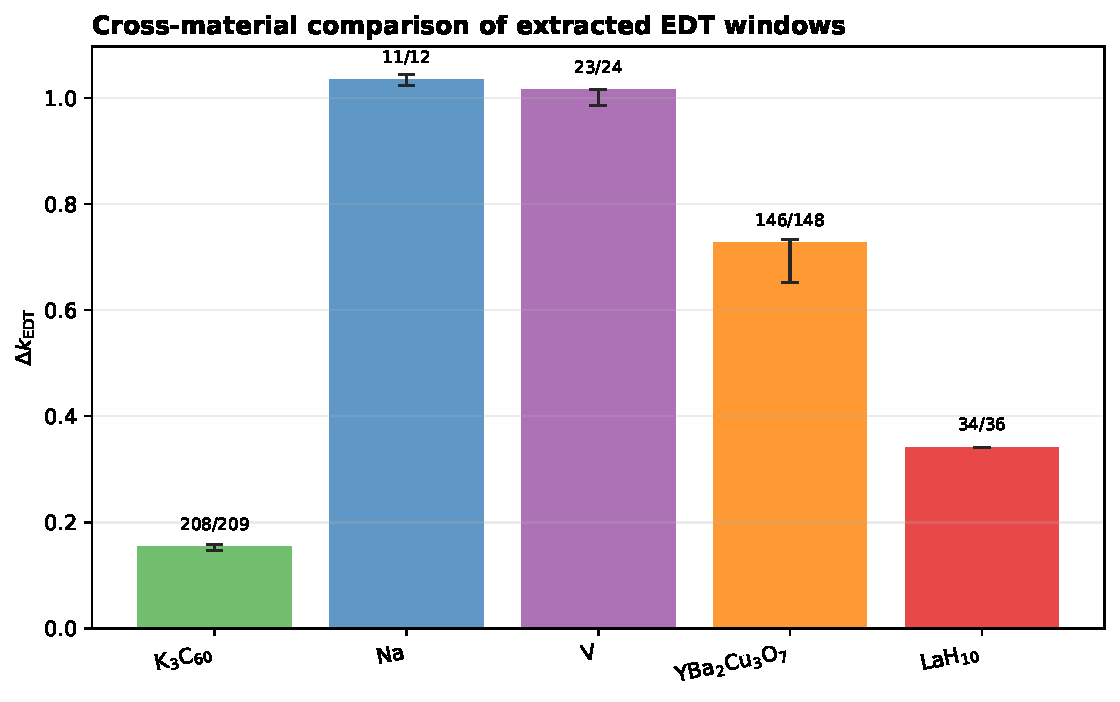
\includegraphics[width=0.72\linewidth]{figs/figure1_material_summary.pdf}
\caption{
\textbf{Cross-material summary of extracted EDT-window widths.}
The bar heights show the residual-defined $\Delta k_{\mathrm{EDT}}$ values extracted from the selected representative branch pairs in K$_3$C$_{60}$, Na, V, YBa$_2$Cu$_3$O$_7$, and LaH$_{10}$, while the error bars show bootstrap confidence intervals from the local quadratic-fit procedure. The fulleride reference remains narrow, the selected Na and V metallic pairs show broader windows, and the selected YBa$_2$Cu$_3$O$_7$ and LaH$_{10}$ subsets remain more localized. Detailed branch-resolved panels for each material are provided in the SI.
}
\label{fig:materials_summary}
\end{figure*}

\begin{figure*}[t]
\centering
\includegraphics[width=0.92\linewidth]{figs/Figure2.pdf}
\caption{
%\textbf{Data-driven identification of the Entanglement-Dynamic Topology (EDT) regime in K$_3$C$_{60}$.}
%(a) Electronic band structure along a high-symmetry path, showing paired bands in the vicinity of the Fermi level.
%(b) Curvature of band energies with respect to the control coordinate, revealing regions of enhanced second-order response associated with non-adiabatic coupling.
%(c) Local quadratic fits to paired curvature branches near the crossing region, demonstrating the emergence of a consistent effective curvature scale $k_0$ within a finite interval.
%(d) Extracted EDT window $\Delta k_{\mathrm{EDT}}$, defined as the momentum region over which the paired curvature branches admit a stable local quadratic description. Together, these panels establish an operational criterion for EDT: a finite momentum-space regime in which curvature structure is coherent, paired, and locally quadratic, indicating the presence of structured, interacting, topological, and dynamical quantum resources.
\textbf{Data-driven identification of the EDT regime in K$_3$C$_{60}$.}
(a) Curvature of band energies near a crossing, showing localized regions of enhanced second-order response. 
(b) Residual analysis defining the validity of local quadratic fits for paired curvature branches. 
(c) Local quadratic structure characterized by an intrinsic scale $k_0$ and a core region $\Delta k_{\mathrm{core}}$. 
(d) Definition of the EDT window $\Delta k_{\mathrm{EDT}}$, the finite momentum interval over which paired curvature branches remain coherent and admit a stable quadratic description. 
This window defines a data-driven criterion for identifying structured quantum resource manifolds in real materials.
}
\label{fig:k3c60_edt}
\end{figure*}


\begin{figure*}[t]
  \centering
  \includegraphics[width=0.98\linewidth]{figs/figure3_edt_regime_panel.pdf}
\caption{\textbf{Finite EDT regime from loop-controlled dynamics.}
(a) OTOC map $C_{\mathrm{OTOC}}(t,\lambda)$ showing loop-induced operator spreading. 
(b) Alignment of OTOC amplitude summaries with the long-time correlator $C_\infty$. While operator spreading increases with loop strength, $C_\infty$ decreases at large $\lambda$, and their overlap defines a finite EDT window. 
(c) OTOC time-structure metrics demonstrating temporally organized dynamics within the same interval. 
(d) Combined EDT phase score, which exhibits a clear maximum at intermediate loop strength. 
(e) Phase classification separating local, EDT, and overdriven regimes. 
(f) Scaling of the optimal loop strength $\lambda^\star$ under variation of $h_x$, demonstrating robustness of the EDT regime.
        }
  \label{fig:fig3_edt_regime}
\end{figure*}


\begin{figure*}[t]
  \centering
  \includegraphics[width=0.80\linewidth]{figs/demo_edt_gyro_trotter_4q_plaquette_otoc.pdf}
\caption{\textbf{Scaling, complexity, and hardware relevance of the EDT regime from 4-qubit plaquette Trotter realization of the EDT gyroscope model.}
(a) Optimal loop strength $\lambda^\star$ under variation of the transverse field $h_x$, showing that the EDT regime is stable over a finite parameter range. 
(b) Peak EDT score $S^\star_{\mathrm{EDT}}$, which exhibits non-monotonic dependence on $h_x$, reflecting competition between operator spreading and long-time correlation. 
(c) Circuit depth and gate count versus evolution time for the Trotterized implementation, showing predictable scaling. 
(d) Observable and OTOC errors versus time, demonstrating that approximation errors remain controlled in the relevant regime. 
(e) Optimal loop strength $\lambda^\star$ versus Trotter budget, showing insensitivity to compilation depth. 
(f) Peak EDT score versus Trotter budget, demonstrating robustness of the EDT regime under approximate circuit implementation.
	}
  \label{fig:si_4q_plaquette_trotter}
\end{figure*}

\begin{figure*}[t]
  \centering
  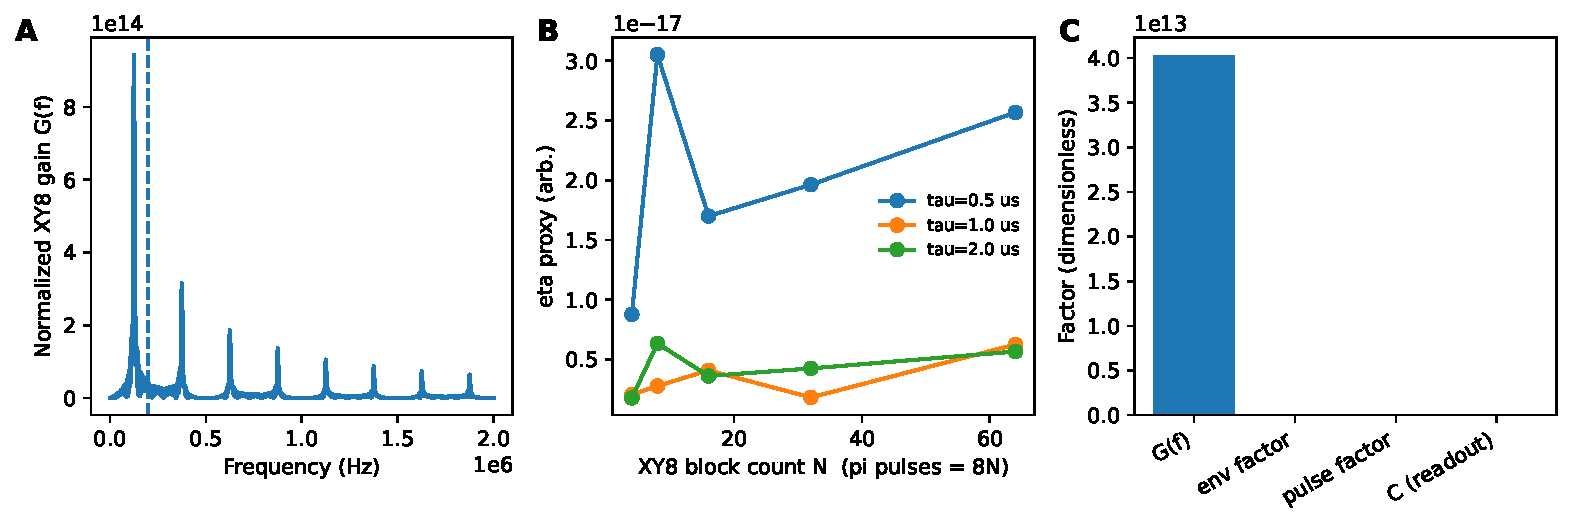
\includegraphics[width=0.90\linewidth]{figs/fig_xy8_qre_nv.pdf}
\caption{\textbf{Quantum resource engineering in NV-center sensing.}
(A) Filter response function $G(f)$ for an XY8 sequence, showing frequency-selective amplification. 
(B) Sensitivity proxy as a function of pulse number $N$ and spacing $\tau$, demonstrating a finite optimal regime. 
(C) Decomposition of sensing performance into resource factors, including filter gain, environmental coherence, pulse fidelity, and readout contrast. 
These results show that optimal sensing arises from a structured balance of competing quantum resources, providing an experimental realization of the EDT regime.
        }
  \label{fig:fig5_nvdemo}
\end{figure*}

%\begin{figure*}[t]
%  \centering
%  \includegraphics[width=0.62\textwidth]{figs/demo_edt_gyro_trotter_4q_circuit_example.pdf}
%\caption{\textbf{4-qubit plaquette Trotter realization of the EDT gyroscope toy model.}
%\textbf{Bottom,} Representative first-order Qiskit Trotter circuit for the four-qubit plaquette model.}
%  \label{fig:si_4q_plaquette_trotter_circuits}
%\end{figure*}

%\section*{Figure Index}

%\textbf{Main Text Figures}

%\begin{itemize}
%\item \textbf{Figure 1:} Conceptual framework of Entanglement--Dynamic Topology (EDT), illustrating the roles of symmetry, interaction, topology, and dynamics.
%\item \textbf{Figure 2:} Data-driven identification of the EDT regime in K$_3$C$_{60}$ via curvature-resolved band structure.
%\item \textbf{Figure 3:} Emergence of the EDT regime in a minimal dynamical model, showing structured operator spreading and persistent correlations.
%\item \textbf{Figure 4:} Scaling and implementation analysis, demonstrating robustness of the EDT regime under circuit approximations.
%\item \textbf{Figure 5:} Experimental realization of the EDT principle in NV-center sensing, showing finite optimal regimes in control space.
%\end{itemize}
%
%\vspace{1em}
%
%\textbf{Supplementary Figures}
%
%\begin{itemize}
%\item \textbf{Figure S1:} Curvature and degeneracy removal in Na.
%\item \textbf{Figure S2:} Curvature structure in V.
%\item \textbf{Figure S3:} Extended curvature structures defining the EDT regime in K$_3$C$_{60}$.
%\item \textbf{Figure S4:} Anisotropic curvature structures in YBa$_2$Cu$_3$O$_7$.
%\item \textbf{Figure S5:} Strong curvature response in LaH$_{10}$.
%\item \textbf{Figure S6:} Temperature-dependent band structure and degeneracy lifting in Nb.
%\end{itemize}
%\bibliographystyle{unsrt}
%\bibliography{references}

\end{document}
